\section{Visibility variance}
\label{app:Vrms}

Here we derive the variance of the visibility for an interferometric array of two antennas separated by a baseline $\vec{b}=(b_x,b_y)$, each with an effective collecting area $A_e$, observing a single element in the $uv$ plane for time duration $t_1$, with total bandwidth $\Delta \nu = \nu_\text{max}-\nu_\text{min}$. We choose notation that is consistent with the rest of this Paper, and adapted to the purpose of discussing measurement of a cosmological signal (as opposed to the traditional context of radio imaging). However, similar derivation can be found in the radio astronomy literature (see, e.g., Refs.~\cite{2001isra.book.....T,1986sicn.book.....P}), and in the literature discussing forecasts for 21--cm experiments (see, e.g., Refs.~\cite{2008PhRvD..78b3529M,2009astro2010S..82F,2014ApJ...782...66P,2007ApJ...661....1B,2008PhRvL.100i1302K,2008PhRvD..78b3529M}).

A schematic of the experimental setup considered here is shown in Fig.~\ref{fig:2antennae}. Modes with frequencies that differ by less than $1/t_1$ cannot be distinguished, and modes with frequencies in each interval $1/t_1$ are collapsed into a discrete mode with frequency $\nu_n = n/t_1$, where $n\in Z$. Thus, the number of measured (discrete) frequencies is $N_\nu=t_1\Delta \nu$. Electric field induced in a single antenna is
\beq
E(t) = \sum_{n}^{N_\nu}\widetilde{E}(\nu_n)e^{2\pi i\nu_nt},
\eeq
while the quantity an interferometer measures is the correlation coefficient between the electric field $E_i$ in one and the electric field $E_j$ in the other antenna, as a function of frequency,
\beq
\rho_{ij}(\nu) \equiv \frac{\langle \widetilde{E}^*_i(\nu)\widetilde E_j(\nu)\rangle}{\sqrt{\langle |\widetilde{E}_i(\nu)|^2\rangle\langle|\widetilde E_j(\nu)|^2\rangle}}.
\label{eq:rho_ij}
\eeq

Let us now assume that 
\beq
\bga
\langle \widetilde{E}^*_i(\nu_n)\widetilde E_j(\nu_m)\rangle=\sigma(\nu)^2\delta_{mn}.
\ega
\label{eq:var_ReE}
\eeq
In the following, for clarity, we omit the dependence on $\nu$.  The real (or imaginary) part of $\rho$ has the following variance
\beq
\bga
\text{var}(Re[\rho_{ij}]) 
\frac{1}{2N_\nu} = \frac{1}{2t_1\Delta \nu}.
\ega
\label{eq:var_Rerho}
\eeq

Before continuing, let us take a brief digression to show that the above formula implicitly assumes that the electric fields in the two antennas have a very weak correlation, $\rho\ll 1$. Consider two random Gaussian variables, $x$ and $y$, both with zero mean values, where $\text{var(x)}\equiv\langle(x-\langle x\rangle)^2\rangle = \langle x^2\rangle - \langle x \rangle^2=\langle x^2\rangle$, and similarly for $y$. Their correlation coefficient is $\rho\equiv \frac{\langle xy\rangle}{\sqrt{\langle x^2\rangle \langle y^2\rangle}}$. In this case, the following is true
\beq
\bga
\text{var}(xy) = \langle x^2y^2\rangle -  \langle xy \rangle^2 = 
\langle x^2\rangle \langle y^2\rangle + \langle xy\rangle^2\\
=\langle x^2\rangle \langle y^2\rangle+\rho^2\langle x^2\rangle\langle y^2\rangle=\text{var}(x)\text{var}(y)(1+\rho^2),
\ega
\eeq
so that when $\rho$ is small, $\text{var}(xy)=\text{var}(x)\text{var}(y)$, which was assumed in the first equality of \eq{\ref{eq:var_Rerho}}.

Resuming the derivation, if different frequencies are uncorrelated, the result of \eq{\ref{eq:var_Rerho}} implies
\beq
\langle|\rho_{ij}(\nu)|^2\rangle = \frac{1}{t_1\Delta \nu}.
\label{eq:var_rho}
\eeq
\begin{figure}
\centering
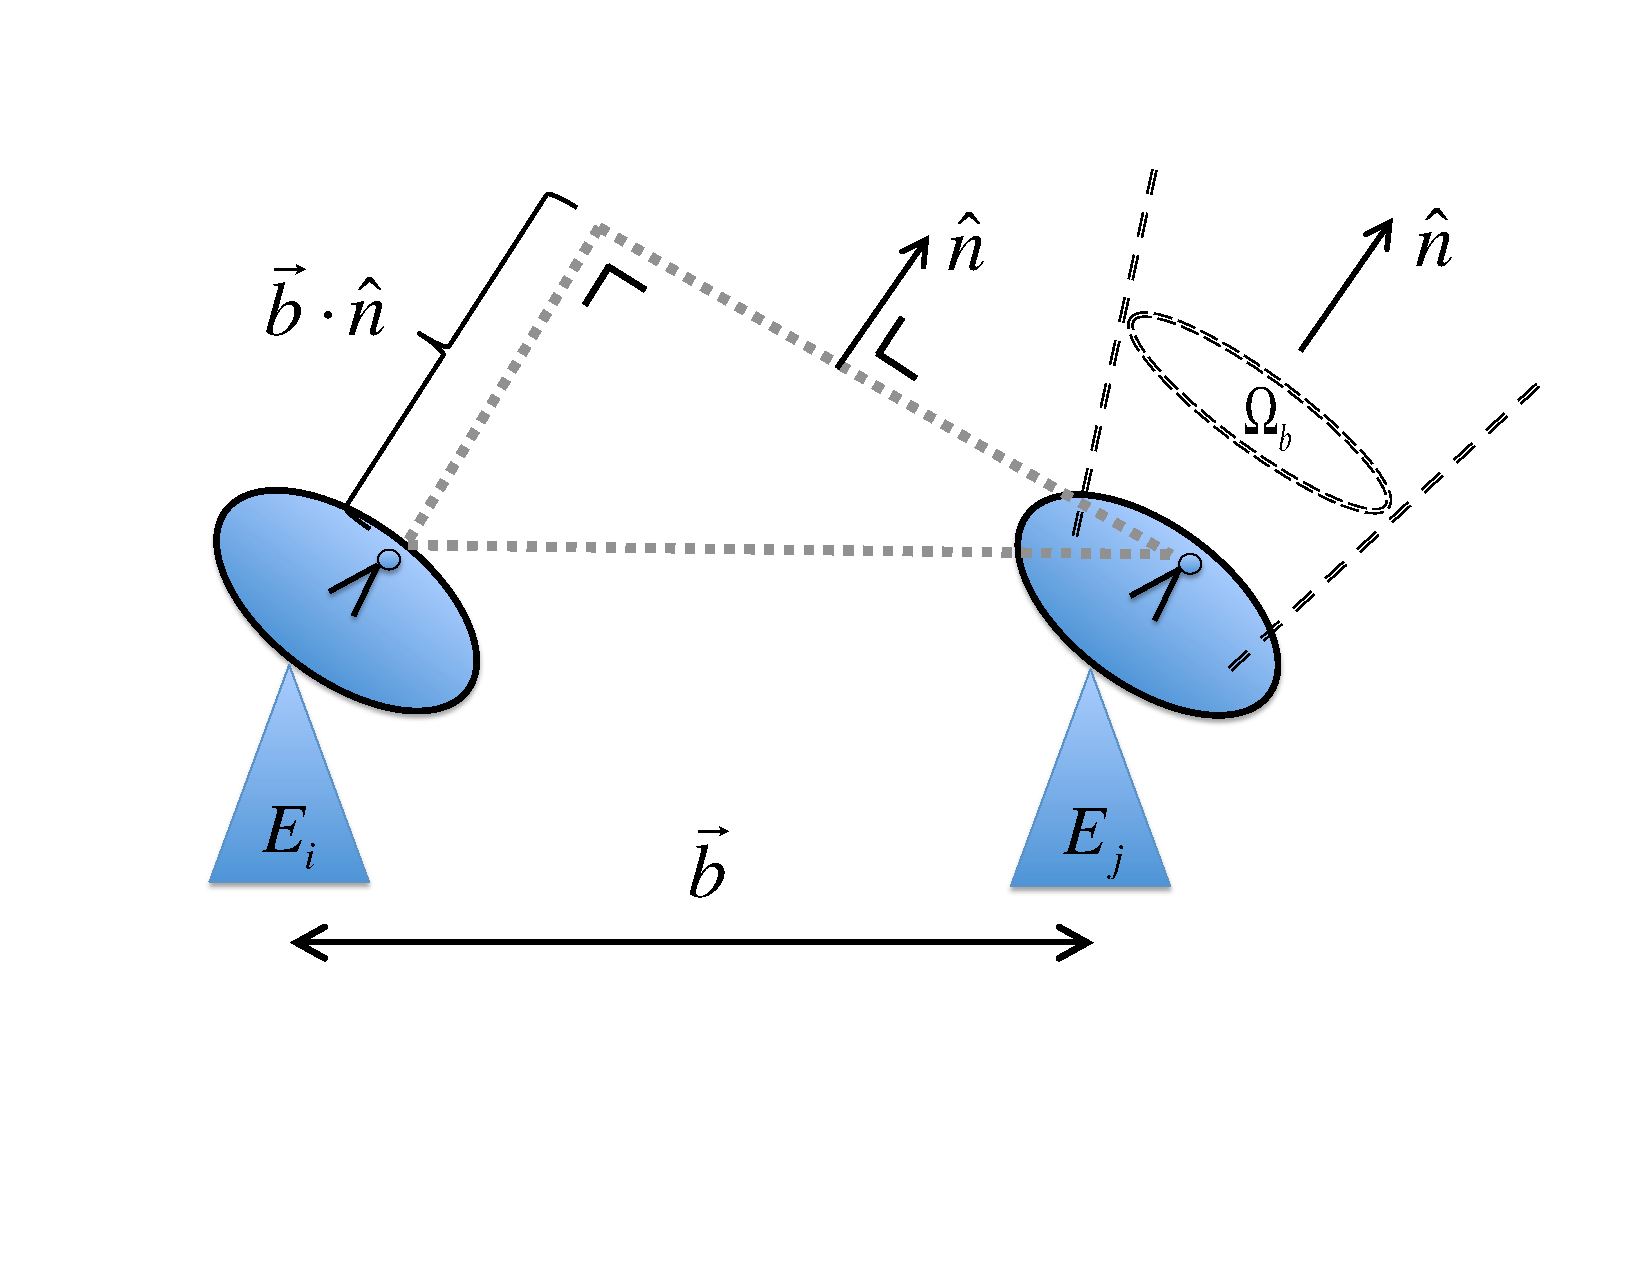
\includegraphics[width=.5\textwidth,keepaspectratio=true]{2antennae.pdf}
\caption{Schematic of a two-antenna interferometer.\label{fig:2antennae}}
\end{figure}

The final step requires a relation between intensity on the sky $\mathcal{I}(\theta_x,\theta_y, \nu)$ (within the beam solid angle $\Omega_\text{beam}$, centered on the direction ${\bf{\widehat n}}=(\theta_x,\theta_y)$) and the electric fields measured in the two antennas,
\beq
\bga
\langle \widetilde{E}_i^*(\nu)\widetilde{E}_j(\nu)\rangle \propto \int_{\Omega_\text{beam}} d\theta_xd\theta_y\mathcal{I}(\theta_x,\theta_y,\theta_\nu)\\
\times e^{ i\frac{2\pi\nu}{c}(b_x\theta_x + b_y\theta_y)  }R(\theta_x,\theta_y),
\ega
\label{eq:E_vs_mathcalI}
\eeq
where $R(\theta_x,\theta_y)$ is the antenna response function (the shape of the beam in the sky), which we will assume to be unity. Furthermore, $\frac{2\pi\nu}{c}(b_x\theta_x + b_y\theta_y)\equiv {2\pi}(u\theta_x + v\theta_y)$ is the phase delay between the two antennas (position in the $uv$ plane measures the phase lag between the two dishes in wavelengths). The coefficient of proportionality in the above Equation is set by various instrumental parameters and is not relevant for our purposes. From \eq{\ref{eq:rho_ij}}, it follows that
\beq
\rho_{ij}(\nu) = \frac{\int_{\Omega_\text{beam}}d\theta_xd\theta_y\mathcal{I}(\theta_x,\theta_y,\theta_\nu)e^{2\pi i(u\theta_x+v\theta_y)}}{\int_{\Omega_\text{beam}}d\theta_xd\theta_y\mathcal{I}(\theta_x,\theta_y,\theta_\nu)},
\label{eq:rho_mathcalI}
\eeq
where the denominator in the above formula approximately integrates to (for a small beam)
\beq
\int_{\Omega_\text{beam}}d\theta_xd\theta_y\mathcal{I}(\theta_x,\theta_y,\theta_\nu) \approx
\Omega_\text{beam} \mathcal{I}(\theta_x,\theta_y,\theta_\nu).
\label{eq:rho_denominator}
\eeq
We can now use the approximate expression for the resolution of a single dish,
\beq
\Omega_\text{beam} = \frac{\lambda^2}{A_e},
\label{eq:Omegab}
\eeq
the Rayleigh--Jeans law (or the definition of the brightness temperature),
\beq
\mathcal{I}(\theta_x,\theta_y,\theta_\nu) = \frac{2k_BT_\text{sky}}{\lambda^2},
\label{eq:I_Tsky}
\eeq
and note that the numerator in \eq{\ref{eq:rho_mathcalI}} matches the definition of visibility from \eq{\ref{eq:visibility}}, to get 
\beq
\rho_{ij}(\nu) = \frac{A_e}{2k_BT_\text{sky}}\mathcal{V}(u,v,\theta_\nu).
\label{eq:rho_V}
\eeq

Combining Eq.~(\ref{eq:rho_V}) and Eq.~(\ref{eq:var_rho}), we get the final result of this derivation,
\beq
\bga
\langle|\mathcal{V}(u,v,\theta_\nu)|^2\rangle 
=\frac{1}{\Omega_\text{beam}}\left(\frac{2k_BT_\text{sky}}{A_e\sqrt{t_1\Delta \nu}}\right)^2\\
\times\delta_D(u-u')\delta_D(v-v')\delta_{\theta_\nu\theta_{\nu'}},
\ega
\label{eq:Vrms_final}
\eeq
where the visibility $\mathcal{V}$ is a complex Gaussian variable, centered at zero, and uncorrelated for different values of its arguments, and the factor of $\Omega_\text{beam}$ came from converting from Kronecker delta to a  Dirac delta function. 

It should be noted that we considered the contribution to the visibility from the noise only (the system temperature + the foreground sky temperature, in the absence of a signal); in the presence of a signal, $T_\text{sky}$ should be the sum of the signal and the noise temperatures.
